% !TEX root = ../Vorlage_DA.tex

%	########################################################
% 				Entwurf
%	########################################################


%	--------------------------------------------------------
% 	Überschrift, Inhaltsverzeichnis
%	--------------------------------------------------------
\chapter{Umsetzung}

%	--------------------------------------------------------
% 	Hardware
%	--------------------------------------------------------
\section{Hardware}

\subsection{LM75A}\label{ref:LM75A}

    Der LM75A ist ein Temperatursensor, welcher via I$^2$C kommuniziert. In der folgenden Abbildung \ref{fig:LM75A} ist er zu sehen.

    \begin{figure}[H]
        \centering
        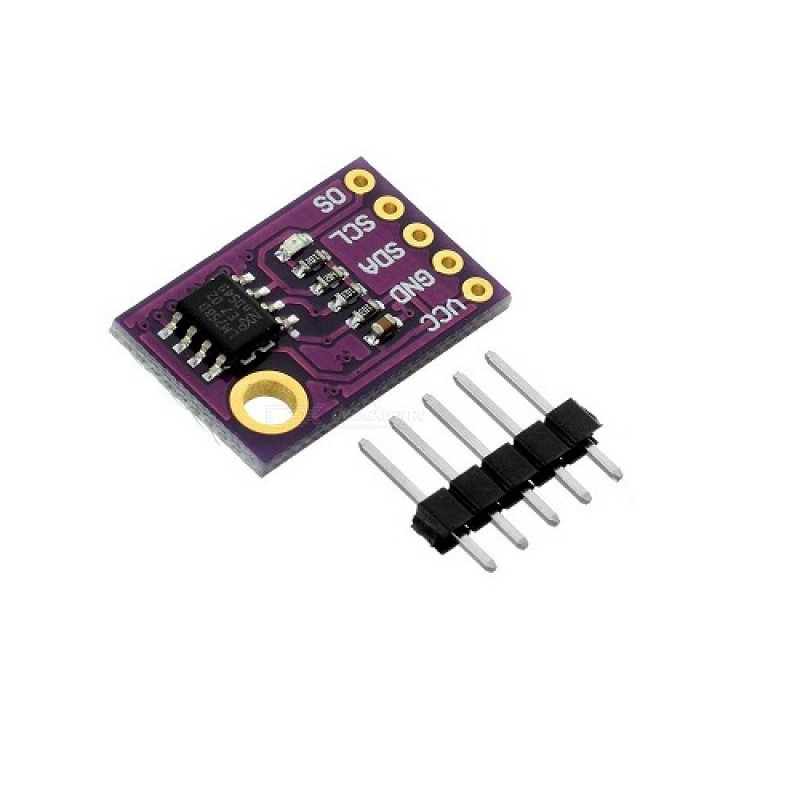
\includegraphics[width=0.5\textwidth]{./media/images/lm.jpg}
        \caption{LM75A\cite{bib:LM75A}}
        \label{fig:LM75A}
    \end{figure}

    Die Messung der Temperatur ist eine der grundlegendsten Funktionen, welche eine Wetterstation können soll. Zusätzlich ist der LM75A mit einem Durchmesser von 23mm sehr klein und billig in der Anschaffung. 
    
    Um Störgrößen zu vermeiden, wurde ein kleiner Kondensator mit 1 $\mu F$, zwischen Versorgung und Ground verbaut. 

\pagebreak

\subsection{ESP8266}\label{ref:ESP8266}

    \begin{figure}[H]
        \centering
        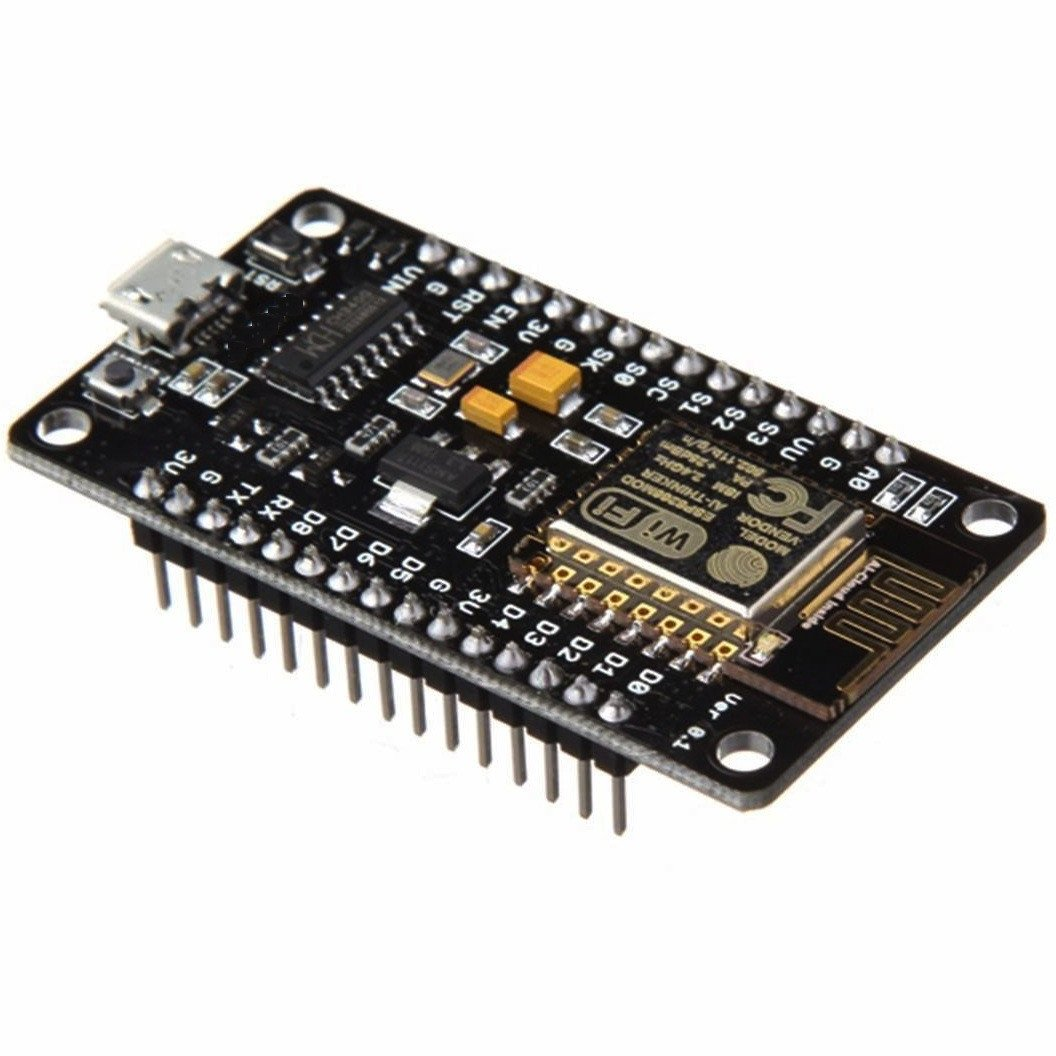
\includegraphics[width=0.3\textwidth]{./media/images/ESP8266.jpg}
        \caption{ESP8266\cite{bib:ESP8266}}
        \label{fig:ESP8266}
    \end{figure}

    Angefangen wurde das Projekt mit dem ESP8266. Dieser ist ein Mikrocontroller, welcher unter Arduino spielend leicht programmierbar ist. Positive Aspekte dessen sind, dass es viele stabile Bibliotheken gibt, welche von vielen Nutzern verwendet werden. Nur ist der ESP8266 unbrauchbar geworden, als es um energiesparendere Wege ging. So musste dann ein neuer Mikrocontroller verwendet werden (siehe \ref{ref:ESP32}).

\subsection{ESP32} \label{ref:ESP32}

    Der ESP32 ist ein Mikrocontroller aus dem Hause Espressif. Er eignet sich ideal für IoT-Projekte (siehe: \ref{ref:IoT}), da er WLAN und Bluetooth an Bord hat. Außerdem besitzt er einen Dual-Core Prozessor, welcher für erhöhte Energie-Effizienz ausgelegt ist. 
    
    \begin{flushright}
            \cite{bib:ESP32Erw}
    \end{flushright}

    \begin{figure}[H]
        \centering
        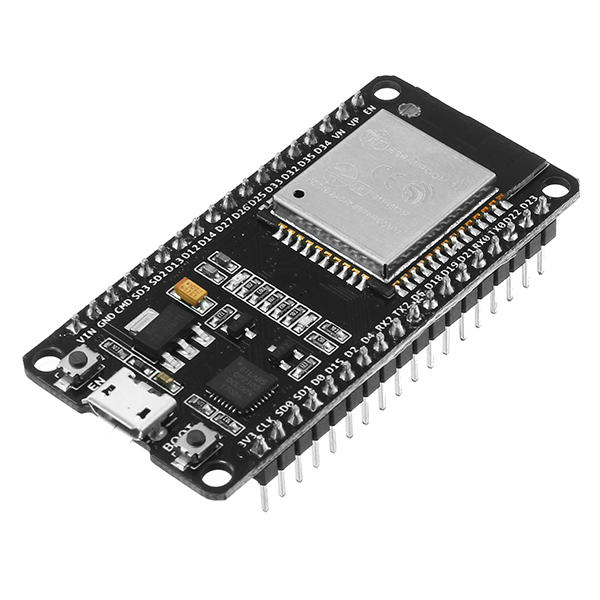
\includegraphics[width=0.3\textwidth]{./media/images/ESP32.jpeg}
        \caption{ESP32 \cite{bib:ESP32}}
        \label{fig:ESP32}
    \end{figure}

    Nachdem der ESP8266 (siehe: \ref{ref:ESP8266}) nicht genügend Energie-effizient war,  ist der ESP32 als neuer Controller ausgewählt worden. Dieser hat nämlich einen Deep-Sleep Modus \ref{ref:DeepSleep} integriert. Probleme hat es mit dem ESP32 jedoch auch gegeben. Viele Bibliotheken, welche es für den ESP32 gibt, sind nicht zuverlässig. Oft musste bei diesen für das eigene Projekt nachgebessert werden. 
    
\pagebreak

\subsection{GPS-Modul}\label{ref:Beitian}

    Der u-blox M8030-KT ist ein GPS-Empfänger, welcher über Serielle Schnittstelle angesprochen wird. In diesem Projekt ist er in einem Modul von Beitian verbaut (siehe Abbildung \ref{fig:Beitian}). Über HardwareSerial.h wird der empfangene Datenstrom des GPS-Empfängers ausgelesen. Dieser Datenstrom kann dann mithilfe der Bibliothek „TinyGPS++.h“ verwertet werden.
    
    \begin{figure}[H]
        \centering
        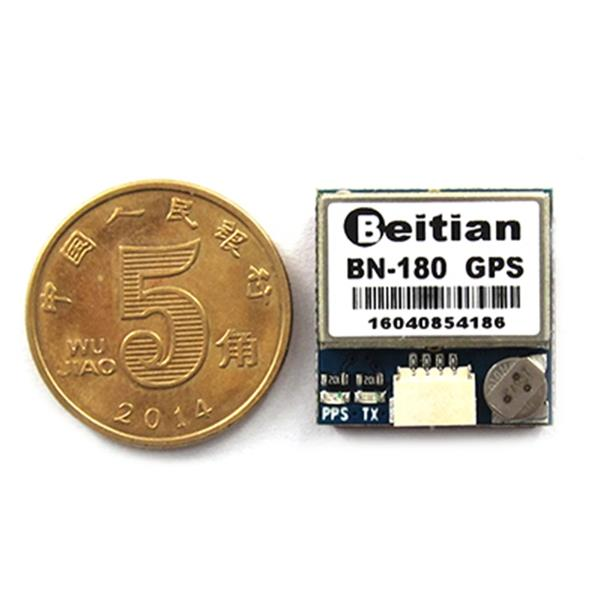
\includegraphics[width=0.4\textwidth]{./media/images/GPS.jpg}
        \caption{Beitian BN-180 im Vergleich zu einer Münze \cite{bib:Beitian}}
        \label{fig:Beitian}
    \end{figure}
    
\subsection{Real-Time Clock}\label{ref:RTC}

    Die Echtzeituhr DS1307 ist ein Modul zum Zählen der Zeit. Sie hat einen integrierten Speicher und ist sehr Energie-effizient. Wenn die Echtzeituhr nicht über den Controller versorgt wird, gibt es die Möglichkeit, eine Batterie zu platzieren. Die Kommunikation mit dem Controller verläuft über I$^2$C.  

    \begin{figure}[H]
        \centering
        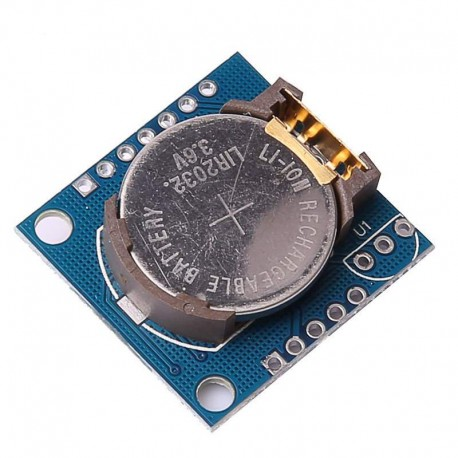
\includegraphics[width=0.3\textwidth]{./media/images/DS1307.jpg}
        \caption{DS1307 Real-Time Clock \cite{bib:DS1307}}
        \label{fig:DS1307}
    \end{figure}
    
    Der ESP32 hat eigentlich bereits eine Real-Time Clock verbaut. Nur ist diese nicht präzise genug und verfälscht die Zeit auf lange Sicht. Deswegen wurde sich für den DS1307 entschieden. 

\pagebreak

%	--------------------------------------------------------
% 	Realisierte Lösungen
%	--------------------------------------------------------
\section{Software}

    \subsection{Atom Editor}\label{ref:Atom}
    
        Atom ist ein moderner Texteditor, welcher sich durch verschiedenste Pakete, Bibliotheken und Designs erweitern und modifizieren lässt. Da Atom ein Produkt von GitHub ist, funktioniert die Anbindung daran einwandfrei. Außerdem gibt es eine Menge an nützlichen Tools, wie zum Beispiel die „smarte Autokorrektur“.  
        
        \begin{flushright}
            \cite{bib:AtomTipps}
        \end{flushright}
        
        In der folgenden Abbildung (\ref{fig:Atom}) sieht man einen Screenshot des Atom-Editors. 
    
        \begin{figure}[H]
            \centering
            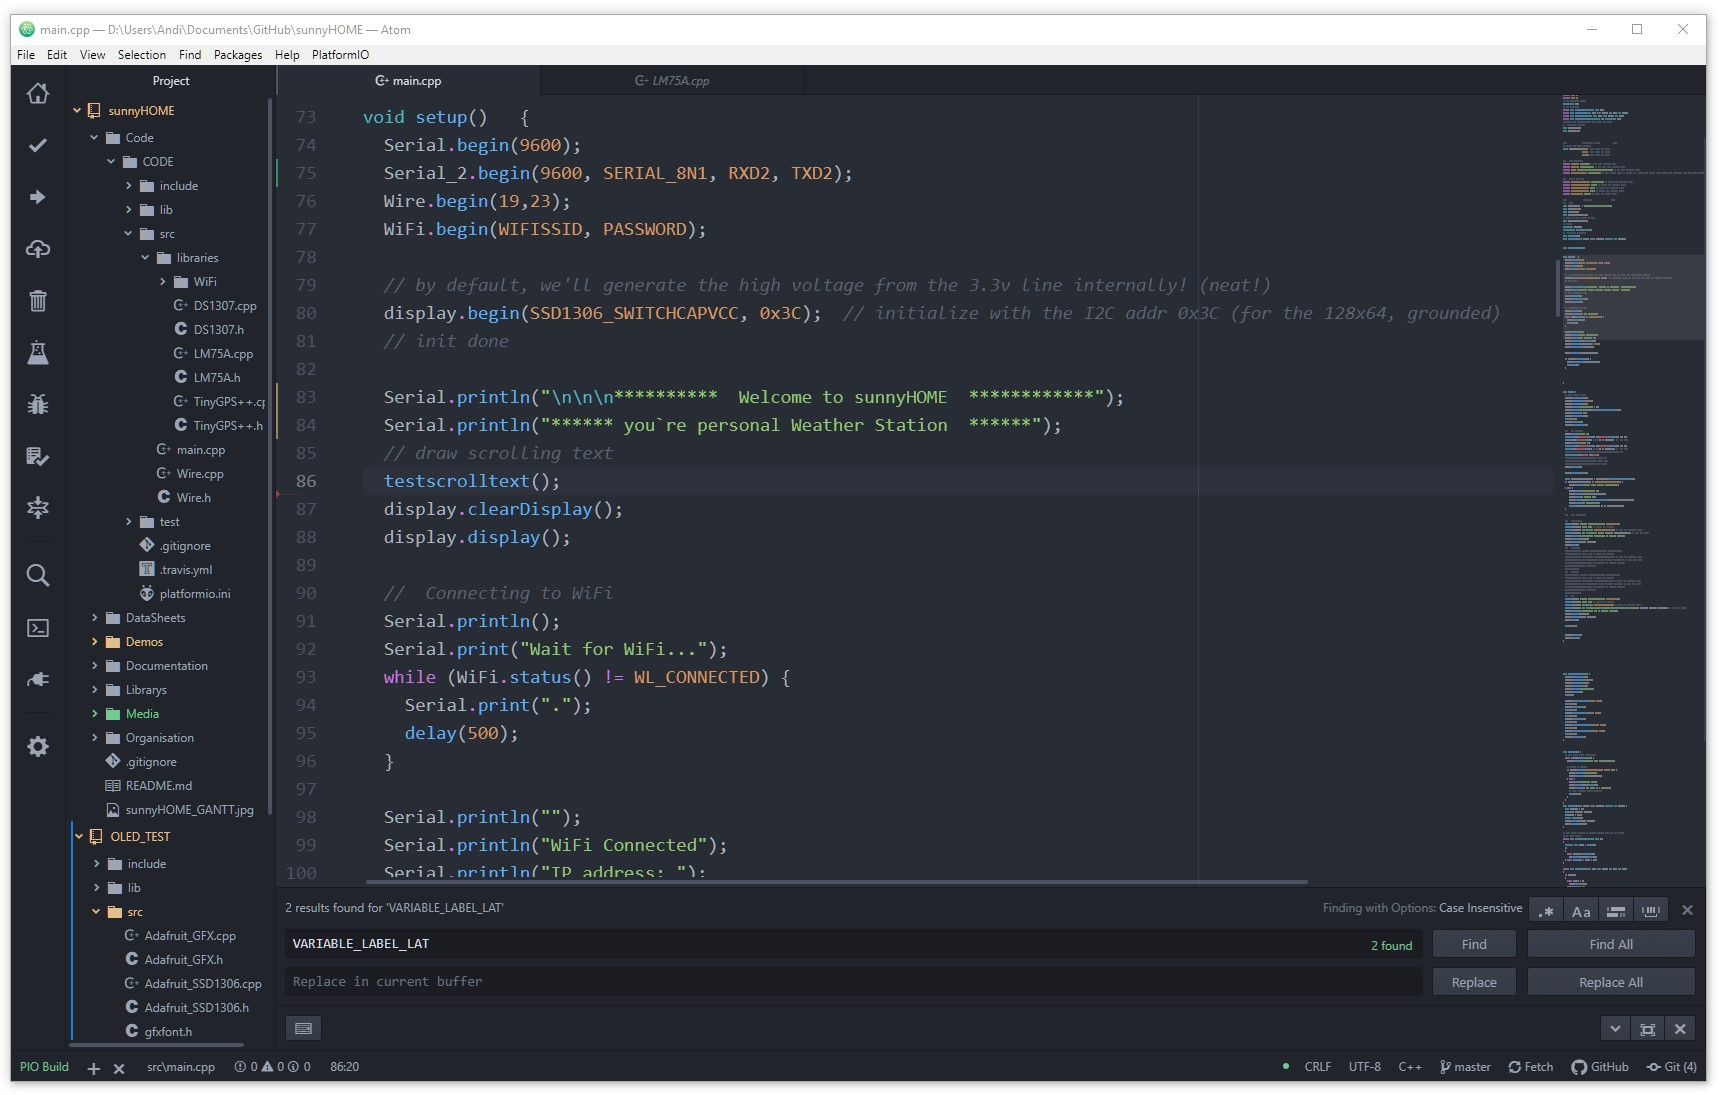
\includegraphics[width=1\textwidth]{./media/images/AtomScreenshot.jpg}
            \caption{Atom Screenshot\cite{bib:Atom}}
            \label{fig:Atom}
        \end{figure}
        
        Gewählt wurde der Atom-Editor, da man ihn auf den meisten Platformen installieren kann und die Installation ebenfalls keine große Hürde ist. Und wie bereits erwähnt wurde, sind die Funktionalitäten dieses Editors sehr praktisch. Um jedoch einen ESP32 programmieren zu können reicht ein gewöhnlicher Texteditor nicht aus. Aus diesem Grund musste das PlatformIO-Paket installiert werden (siehe \ref{ref:PlatformIO}). 
        
    
\pagebreak

    \subsection{PlatformIO}\label{ref:PlatformIO}
    
    PlatformIO ist eine IDE\footnote{Wikipedia-Eintrag: https://de.wikipedia.org/wiki/Integrierte\_Entwicklungsumgebung, 06. April 2019}, welche im speziellen für das Programmieren von Mikrocontrollern gedacht ist. Es lassen sich die geschriebenen Codes auf Fehler überprüfen, man hat die Möglichkeit die geschriebenen Programme mit Kabel oder kabellos auf den Controller zu laden, und ein Serieller Monitor, über welchen man Nachrichten des Mikrocontrollers empfangen kann, ist ebenfalls verbaut.
    
    \begin{figure}[H]
        \centering
        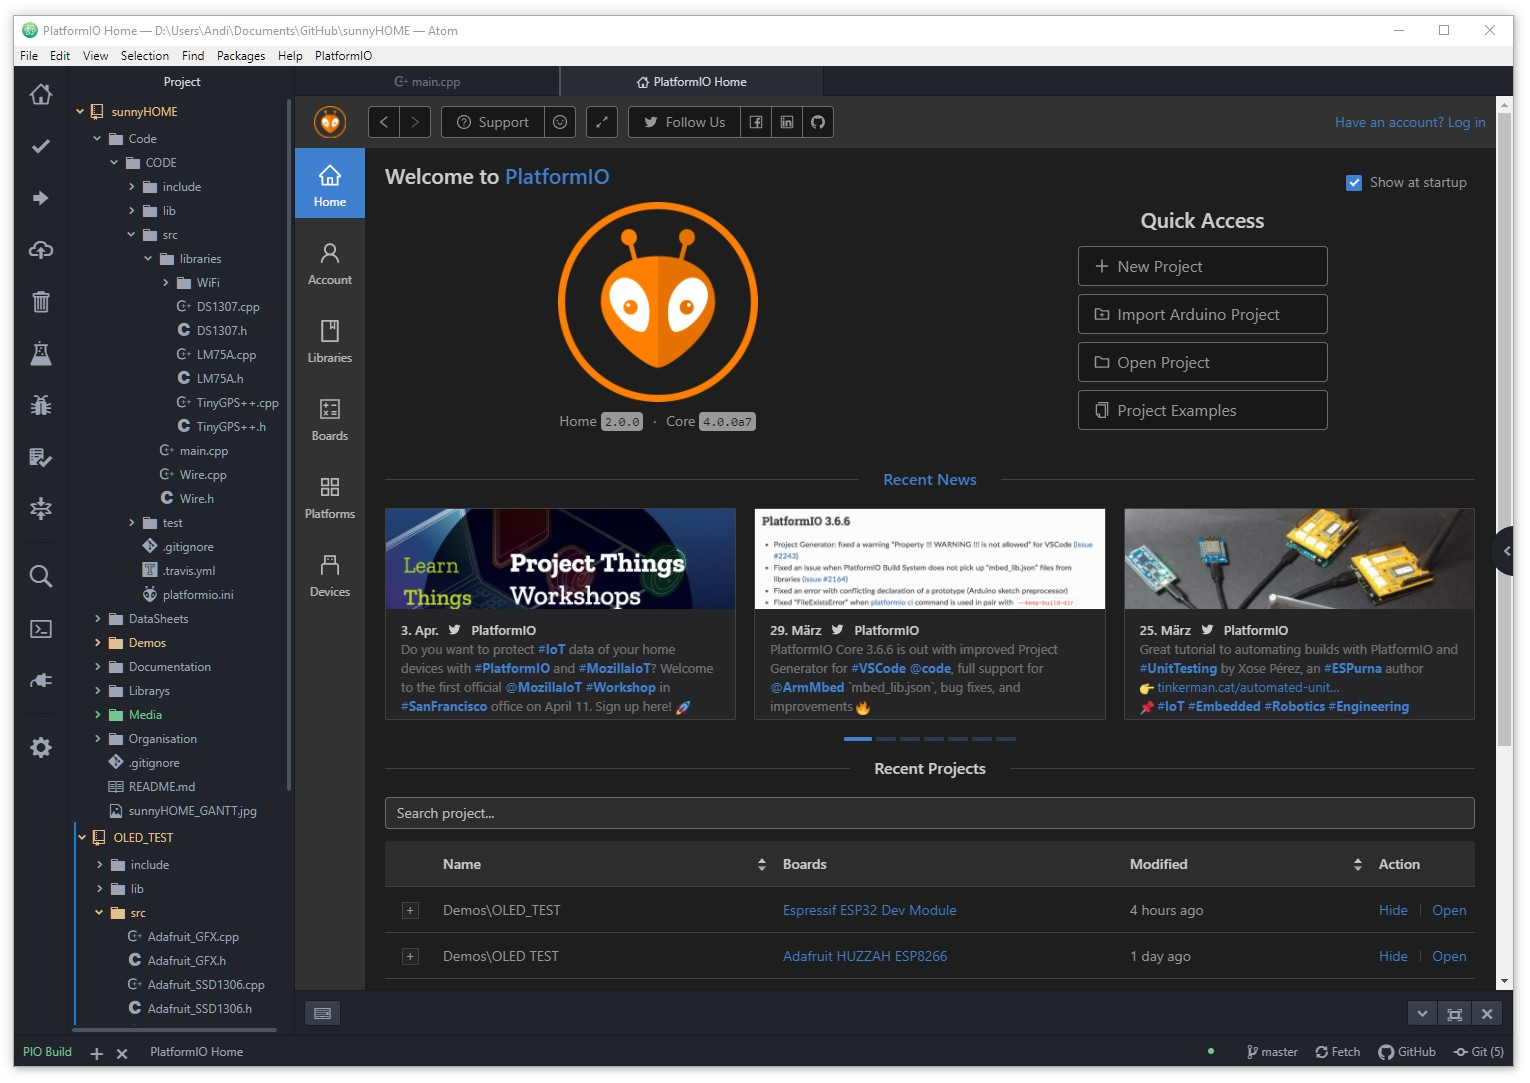
\includegraphics[width=1\textwidth]{./media/images/PlatformIO.jpg}
        \caption{PlatformIO Screenshot\cite{bib:PlatformIO}}
        \label{fig:PlatformIO}
    \end{figure}
    
    Entschlossen wurde sich für diese IDE, da diese eine Lösung für die Programmierung mit Atom (siehe: \ref{ref:Atom}) gewesen ist.
    
    
    
\pagebreak

\subsection{Ubidots \cite{bib:ubidots}}\label{ref:Ubidots}
    
    Ubidots ist ein MQTT-Broker, welcher wie ein Cloud-Service funktioniert. Mit Hilfe von Ubidots lassen sich die Daten eines Mikrocontrollers spielend leicht im Internet publizieren und visualisieren. Man kann sich beispielsweise Statistiken über Temperaturunterschiede der letzten Wochen anzeigen lassen, oder natürlich ebenfalls auf aktuell aufgenommene Daten wie GPS-Standort zugreifen. 
    
    \begin{figure}[H]
        \centering
        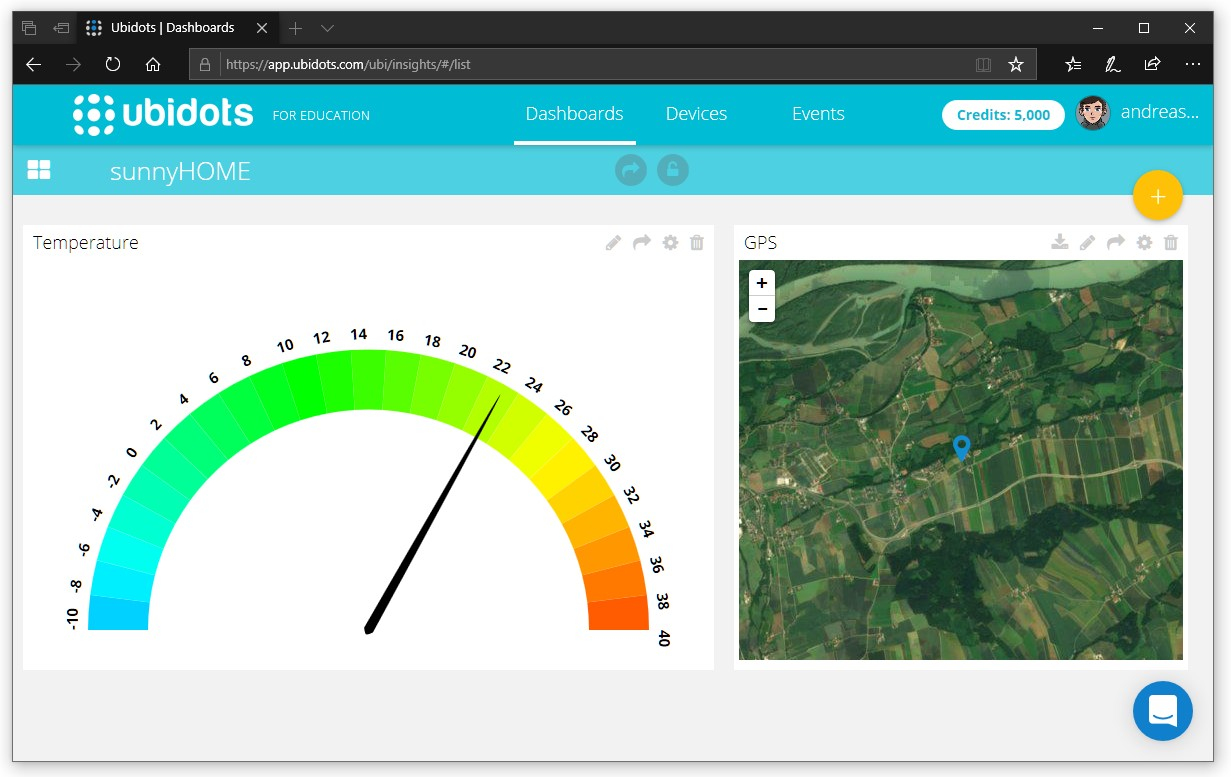
\includegraphics[width=1\textwidth]{./media/images/ubidotsSC.jpg}
        \caption{Ubidots-Dashboard Screenshot\cite{bib:ubidots}}
        \label{fig:ubidots}
    \end{figure}
    
    Zu Beginn des Matura-Projektes, ist noch das Erstellen einer eigenen Website und einer eigenen App geplant gewesen. Da das Projekt schlussendlich doch alleine durchgeführt wurde, musste eine einfachere Lösung gefunden werden. So wurde dann Ubidots als Darstellungs-Plattform gewählt. 

\pagebreak

\section{Bibliotheken}
    \subsection{HardwareSerial.h}
    
        Die „HardwareSerial-Bibliothek“ behandelt die Hardware-Schnittstellen (UART) des ESP32. Grundsätzlich sind am Mikrocontroller drei Schnittstellen verbaut. Die standardmäßige Pinbelegung der Schnittstellen kann jedoch problematisch werden, da dieselben Pins zum Beispiel die Ansteuerung des internen Flashspeichers oder Reseteingänge belegen. Dafür bietet der ESP32 aber eine einfache Lösung: Mit Hilfe der HardwareSerial Bibliothek lassen sich die Hardware-Schnittstellen mit beinahe jedem IO-Pin verbinden.
        \begin{flushright}
            \cite{bib:HWSerial}
        \end{flushright}
        
        In Listing \ref{code:HWSerial} wird die Implementierung der seriellen Schnittstelle des GPS-Moduls gezeigt. Über diese werden im eingeschalteten Modus dauerhaft GPS-Daten an den Controller geliefert. 
        \begin{lstlisting}[
            language=c,
            caption={HardwareSerial Initialisierung },
            label=code:HWSerial
        ]
////                GPS-Reseiver                    ////
HardwareSerial gps(2); // (2) weil UART2

void setup() {
  // Datenrate: 9600 Bit/s, Rx-Pin: 16, Tx-Pin: 17
  gps.begin(9600, SERIAL_8N1, 16, 17); 
}
        \end{lstlisting}
    
    \subsection{Wire.h}
        Die „Wire-Bibliothek“ erlaubt es einem, via I$^2$C zu kommunizieren. Sie hat eine ähnliche Funktionalität wie die „HardwareSerial-Bibliothek“. In dem man die gewünschten Pins in „Wire.begin()“ einfügt, lässt sich die I$^2$C-Kommunikation einstellen. Wenn nichts eingefügt wird, werden die Standard Pins gewählt. 
        
        Nachdem ein ESP32-Devboard während des Jahres kaputt gegangen ist, musste bei dem nächsten ESP32-Board auf die Standard Pin-Belegung verzichtet werden. Aus diesem Grund mussten, wie in Listing \ref{code:Wire} beschrieben, die Pins neu definiert werden. 
        \begin{lstlisting}[
            language=c,
            caption={I2C Konfiguration},
            label=code:Wire
        ]
#include <Wire.h>

void setup() {
  // SDA: 19, SCL: 23
  Wire.begin(19,23); 
}
        \end{lstlisting}
        
        Somit läuft die komplette I$^2$C-Kommunikation über die ausgewählten Pins. Werden jedoch Bibliotheken, welche man für I$^2$C-Bausteine eingebunden hat verwendet, muss aufgepasst werden, dass diese Pin-Belegung nicht verändert wird. 
        
\pagebreak
    
    \subsection{WiFi.h \& PubSubClient.h}
        
        Die ESP32-Bibliothek „WiFi.h“ ist für die Verbindung zum WLAN-Netz verantwortlich. Im folgenden Listing \ref{code:WiFi} ist der Code für die Verbindung zu einem WLAN-Netzwerk zu sehen. Es wird nur das einfügen des WLAN-Namen und WLAN-Passwortes benötigt.
        
        \begin{lstlisting}[
            language=c,
            caption={WLAN Konfiguration},
            label=code:WiFi
        ]
#include <WiFi.h>

void setup() {
  WiFi.begin(WIFISSID, PASSWORD); 
}
        \end{lstlisting}
        
        Um eine Verbindung zu einem MQTT-Broker herzustellen braucht es aber noch mehr. Dazu wird die Bibliothek „PubSubClient.h“(Publish-Subscribe Client) benötigt. Diese ermöglicht es einem, MQTT-Topics zu versenden. Listing \ref{code:payload} zeigt die Publikation des Temperatur-Topics.
        
        \begin{lstlisting}[
            language=c,
            caption={Erstellen der Payload und Publikation der Temperatur},
            label=code:payload
        ]
/**********   Temperatur-Publikation   ***********/
//  hier wird die ID des Ubidots-Gerätes eingetragen
sprintf(topic, "%s%s", "/v1.6/devices/", DEVICE_LABEL);
// payload wird gereinigt
sprintf(payload, "%s", ""); 
//  hier wird die ID der Ubidots-Variable eingetragen
sprintf(payload, "{\"%s\":", VARIABLE_LABEL_TEMP);
//  hier wird der String mit der Temperatur eingetragen
sprintf(payload, "%s {\"value\": %s}}", payload, str_temperature);
//  Datenpaket wird versendet
client.publish(topic, payload);
        \end{lstlisting}
        
        Das verschickte Datenpaket (die Payload) sieht folgendermaßen aus:
        \begin{center}
            \{''temperature``: \{''value``: 26.37\}\}
        \end{center}
    
    \subsection{DS1307.h}
    
        Die Bibliothek „DS1307.h“ ist für die RTC (Real-Time Clock, siehe: \ref{ref:RTC}) zuständig. Um die aktuelle Zeit einzutragen, wird die GPS-Zeit mit der RTC-Zeit periodisch synchronisiert. 
        
        In Listing \ref{code:time} ist das Eintragen der GPS-Zeit und des GPS-Datums in die Real-Time Clock zu sehen.  
        
        \begin{lstlisting}[
            language=c,
            caption={Synchronisierung der GPS-Zeit mit der RTC-Zeit},
            label=code:time
        ]
#include <DS1307.h>
RTC_DS1307 rtc;

void setup() {
  rtc.begin()
  //  TinyGPSDate &d ... GPS-Datum, TinyGPSTime &t ... GPS-Zeit
  rtc.adjust(DateTime(d.year(), d.month(), d.day(), t.hour(), t.minute(), t.second()));  
}
        \end{lstlisting}
        
    \subsection{TinyGPS++.h}
    
    Die Bibliothek „TinyGPS++.h“ ist vor allem für eine Sache zuständig: das Übersetzen des ankommenden seriellen Datenstroms des GPS-Receivers (siehe: \ref{ref:Beitian}).
    
    Es gibt jedoch auch einige nützliche Funktionen, welche die Bedienung des GPS-Receivers vereinfachen (siehe: Listing\ref{code:GPSFunct}). 
    
            \begin{lstlisting}[
            language=c,
            caption={TinyGPS++ Funktionen},
            label=code:GPSFunct
        ]
//************   GPS Functions   ************//
//  Entschlüsselt Datenstrom
static void smartDelay(unsigned long ms);
//  Gibt gewünschte Daten als Float im Seriellen Monitor aus 
static void printFloat(float val, bool valid, int len, int prec);
//  Gibt gewünschte Daten als Integer im Seriellen Monitor aus 
static void printInt(unsigned long val, bool valid, int len);
//  Gibt aktuelles Datum und Uhrzeit im Seriellen Monitor aus
static void printDateTime(TinyGPSDate &d, TinyGPSTime &t);
        \end{lstlisting}
        
        
        
        
        Die wichtigste der Funktionen ist die „smartDelay“-Funktion. Sie entschlüsselt den ankommenden seriellen GPS-Datenstrom und packt die entschlüsselten Informationen in die „TinyGPSPlus“-Variable:
        
        \begin{lstlisting}[
            language=c,
            caption={„smartDelay“-Funktion},
            label=code:smartDelay
        ]
static void smartDelay(unsigned long ms)
{
  unsigned long start = millis();
  do
  {
//  Solange ein serieller Datenstrom ankommt, 
//  soll dieser entschlüsselt werden
    while (HWSerialGPS.available())
//  gps ist eine TinyGPSPlus-Variable
      gps.encode(HWSerialGPS.read());
  } while (millis() - start < ms);
}
        \end{lstlisting}
        
        
        
        Damit die Daten über MQTT versendet werden können, müssen sie als Strings gespeichert werden. Es gibt jedoch keine Möglichkeit, die Koordinaten als Strings zu erhalten. Dazu muss die folgende Wandlung gemacht werden: 
  
        \begin{lstlisting}[
            language=c,
            caption={Float zu String Wandlung für MQTT},
            label=code:FloatString
        ]
//      1.Parameter: Breitengrad in float               
//      2.Parameter: Zahl darf 9 Stellen lang sein 
//      3.Parameter: mit maximal 6 Nachkommastellen     
//      4.Parameter: wird in folgende String gewandelt 
dtostrf(gps.location.lat(), 9, 6, str_lat);  //  für MQTT 
dtostrf(gps.location.lng(), 9, 6, str_long); //  für MQTT
        \end{lstlisting}

